\chapter{Cypherpunks escrevem código}
\label{les:20}

\begin{chapquote}{Lewis Carroll, \textit{Alice no País das Maravilhas}}
\enquote{Eu posso ver que você está tentando inventar alguma coisa.}
\end{chapquote}

Grandes ideias não surgem do nada, com o Bitcoin, também foi assim. 
Ele só foi possível combinando muitas inovações e descobertas da matemática, 
física, ciências da computação, e muitas outras áreas. Mesmo sendo um gênio, 
Satoshi não conseguiria inventar o Bitcoin sem estar apoiado sobre os ombros de gigantes.

\begin{quotation}\begin{samepage}
\enquote{Aquele que apenas espera e deseja não interfere ativamente no curso dos eventos e com a criação do próprio destino.}
\begin{flushright} -- Ludwig von Mises\footnote{Ludwig von Mises, \textit{Ação Humana} \cite{human-action}}
\end{flushright}\end{samepage}\end{quotation}
% > <cite>[Ludwig Von Mises]</cite>

Um desses gigantes é o Eric Hughes, um dos fundadores do movimento cypherpunk
e escritor do \textit{O Manifesto dos Cypherpunks}. Em inglês \textit{A Cypherpunk's Manifesto}. 
É difícil imaginar que Satoshi não tenha sido influenciado por esse manifesto. Nele já se falava de muitas coisas que o Bitcoin proporciona e usa, como transações diretas e privadas, dinheiro e moedas eletrônicas, sistemas anônimos e, a defesa de privacidade com criptografia e assinaturas digitais.

\begin{quotation}\begin{samepage}
\enquote{Privacidade é necessária para uma sociedade livre na era eletrônica.
	[...] Já que desejamos privacidade, nós temos que ter certeza que cada parte 
	na transação tenha conhecimento só do que é diretamente necessário para 
	aquela transação [...]
	Assim, privacidade em uma sociedade livre requer sistemas de transação anônima. 
	Até agora, o dinheiro tem sido o principal sistema desse tipo.
	O sistema de transações anônimas não é um sistema de transações secretas. [...]
	Nós os Cypherpunks, estamos dedicados em construir sistemas anônimos. Nós vamos 
	defender a nossa privacidade com criptografia, com sistemas de encaminhamento 
	de e-mails anônimos, com assinaturas digitais, e com dinheiro eletrônico. 
	Os cypherpunks escrevem código.}

\begin{flushright} -- Eric Hughes\footnote{Eric Hughes, O Manifesto dos Cypherpunks \cite{cypherpunk-manifesto}}
\end{flushright}\end{samepage}\end{quotation}

Cypherpunks não se confortam com esperanças e desejos. 
Eles ativamente interferem com os eventos em curso e moldam seu próprio destino. 
Os cypherpunks escrevem código.

Assim, no verdadeiro estilo cypherpunk, Satoshi sentou e começou a escrever código. 
Código que de uma ideia abstrata e provou para o mundo que ela realmente funcionava. 
Código que plantou a semente de uma nova realidade econômica.
Graças a esse código, todo mundo pode verificar que esse sistema novo realmente funciona, 
a cada dez minutos mais ou menos, o Bitcoin provou isso para o mundo e ainda vive.

\begin{figure}
  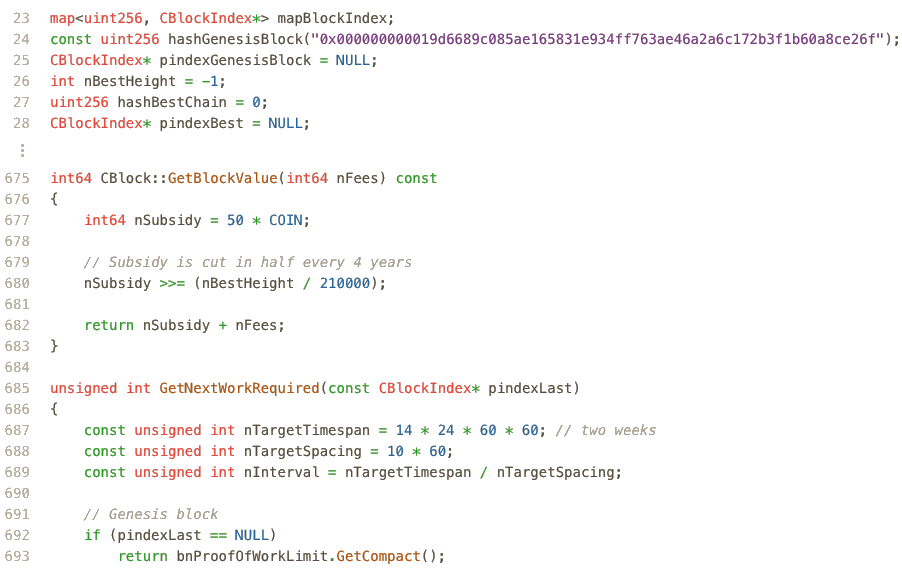
\includegraphics{assets/images/bitcoin-code-white.png}
  \caption{Trechos de código do Bitcoin version 0.1}
  \label{fig:bitcoin-code-white}
\end{figure}

Para ter certeza de que sua inovação transcende a fantasia e vira realidade, Satoshi 
escreveu o código para implementar essa ideia antes de escrever o artigo técnico. 
Ele também fez questão de não atrasar\footnote{\enquote{Nós não devemos atrasar 
		se todos os recursos estão prontos.} 
	-- Satoshi Nakamoto~\cite{satoshi-delay}} qualquer versão para sempre.
	Até porque, \enquote{sempre tem mais uma coisa ser feita.}

\begin{quotation}\begin{samepage}
\enquote{Eu tive que escrever todo aquele código, antes de me convencer que eu podia resolver todo problema, só depois eu escrevi o artigo.}
\begin{flushright} -- Satoshi Nakamoto\footnote{Satoshi Nakamoto, em resposta ao Bitcoin P2P e-cash paper \cite{satoshi-mail-code-first}}
\end{flushright}\end{samepage}\end{quotation}

No mundo de hoje, cheio de promessas de execução duvidosa, um exercício de construção dedicada 
era desesperadamente necessário. Propositalmente, para convencer a si mesmo de que você pode realmente resolver os problemas e, implementar as soluções. 
Todos nós devemos ter como objetivo um pouco mais cypherpunk. 

\paragraph{O Bitcoin me ensinou que cypherpunks escrevem código.}

% ---
%
% #### Down the Rabbit Hole
%
% - [Bitcoin version 0.1.0 announcement][version 0.1.0] by Satoshi Nakamoto
% - [Bitcoin P2P e-cash paper announcement][mail-announcement] by Satoshi Nakamoto
%
% [mail-announcement]: http://www.metzdowd.com/pipermail/cryptography/2008-October/014810.html
% [Ludwig Von Mises]: https://mises.org/library/human-action-0/html/pp/613
% [version 0.1.0]: https://bitcointalk.org/index.php?topic=68121.0
% [not to delay]: https://bitcointalk.org/index.php?topic=199.msg1670#msg1670
% [6]: http://www.metzdowd.com/pipermail/cryptography/2008-November/014832.html
%
% <!-- Wikipedia -->
% [alice]: https://en.wikipedia.org/wiki/Alice%27s_Adventures_in_Wonderland
% [carroll]: https://en.wikipedia.org/wiki/Lewis_Carroll
